\documentclass{article}
\usepackage{graphicx} % Required for inserting images
\usepackage{fullpage}
\usepackage{natbib}
\usepackage{tikz}
\usetikzlibrary{positioning}
\usepackage{color}
\usepackage{graphicx}
\usepackage{booktabs}
\usepackage{multirow}
\usepackage{makecell}
\usepackage{array}
\usepackage{subcaption}
\usepackage{setspace}
\usepackage{float}
\usepackage{tabularx}
\usepackage[round]{natbib}
\usepackage[font={small,it}]{caption}
\usepackage[utf8]{inputenc}
\usepackage{mathtools}
\usepackage{fullpage}
\usepackage{verbatim}
\usepackage{amsfonts,amssymb,amsthm}
\usepackage{url}
\usepackage{authblk}
\usepackage{xcolor}
\usepackage{algorithm}
\usepackage{algorithmic}
\usepackage[colorlinks=true,citecolor=blue]{hyperref}
\bibliographystyle{apalike}
\title{Poisson Approximate Likelihood versus block particle filter for a spatiotemporal measles model}
\author{Kunyang He, Yize Hao and Edward L. Ionides}
\date{\today\\
\eic{DRAFT IN PROGRESS, LOOKING TO CLARIFY THE CALCULATIONS THAT WE NEED TO SECURE THE MAIN ARGUMENT}}

\newcommand\loglik{\lambda}

\newcommand\fproc{f_{\mathrm{proc}}}
\newcommand\fmeas{f_{\mathrm{meas}}}
\newcommand\sproc{s_{\mathrm{proc}}}
\newcommand\smeas{s_{\mathrm{meas}}}

\newcommand\fprocDiscrete{\mathrm{discrete}}
% \newcommand\fprocDiscrete{$f_D$}
\newcommand\fprocEuler{\mathrm{Euler}}
% \newcommand\fprocEuler{$f_E$}
\newcommand\fmeasBinomial{\mathrm{binomial}}
% \newcommand\fmeasBinomial{$f_B$}
\newcommand\fmeasGaussian{\mathrm{Gaussian}}
% \newcommand\fmeasGaussian{$f_G$}

\newcommand\sprocDiscrete{\mathrm{discrete}}
% \newcommand\sprocDiscrete{$s_D$}
\newcommand\sprocEuler{\mathrm{Euler}}
% \newcommand\sprocEuler{$s_E$}
\newcommand\smeasBinomial{\mathrm{binomial}}
% \newcommand\smeasBinomial{$s_B$}
\newcommand\smeasGaussian{\mathrm{Gaussian}}
% \newcommand\smeasGaussian{$s_G$}

\newcommand\PALL{$\mathrm{PAL}_L$} % lookahead PAL
\newcommand\PALV{$\mathrm{PAL}_V$} % vanilla PAL

\newcommand{\bs}{\boldsymbol}

\usepackage{multirow}
\usepackage[dvipsnames]{xcolor}
\newcommand\eic[1]{{\color{Orange} #1}}



\begin{document}

\maketitle

\begin{abstract}
Filtering algorithms for high-dimensional nonlinear non-Gaussian partially observed stochastic processes provide access to the likelihood function and hence enable likelihood-based or Bayesian 
inference for complex dynamic systems.
A novel Poisson approximate likelihood (PAL) filter was introduced by Whitehouse et al. (2023). PAL employs a Poisson approximation to conditional densities, offering a fast approximation to the likelihood function for a certain subset of partially observed Markov process models.
PAL was demonstrated on an epidemiological metapopulation model for measles, specifically, a spatiotemporal model for disease transmission within and between cities. 
At face value, Table~3 of Whitehouse et al. (2023) suggests that PAL considerably out-performs previous analysis as well as an ARMA benchmark model.
We show that PAL does not outperform a block particle filter and that the lookahead component of PAL was implemented in a way that introduces positive bias in the log-likelihood estimates.

\end{abstract}

\section{Introduction}

Investigations of the metapopulation dynamics of measles (i.e., studying how measles infection moves within and between collections of spatially distinct populations) have motivated various methodological innovations for inference on high-dimensional partially observed stochastic processes [REFS].
The analysis by \citet{whitehouse23} (henceforth, WWR) provides a new approach to model-based inference on population dynamics via the Poisson approximate likelihood (PAL) filtering algorithm.
WWR claimed impressive results on both a low-dimensional dengue transmission model and a high-dimensional measles model. 
On close inspection, the dengue results turned out to be overstated \citep{hao24-arxiv} leading to a published correction \citep{whitehouse25-correction}.
However, the measles results remained unchallenged, and our present goal is to revisit that evidence.
In Section~\ref{sec:numerics} we show by direct numerical experimentation that the WWR implementation of PAL has substantial positive bias in the log-likelihood estimate, and so the use of log-likelihood to support the use of the method is flawed.
While doing this, we show that a widely applicable block particle filter (BPF) is adequate on this problem.
In Section~\ref{sec:theory} we explain theoretically how the positive bias for PAL arises as a result of the lookahead mechanism included in the implementation of PAL for this model.
The lookahead mechanism was not used by WWR for the dengue analysis since its purpose was to address numerical issues involved in high-dimensional filtering.
Section~\ref{sec:conclusion} is a concluding discussion.

For our current purposes, we do not have to delve into the details of the measles data and model, so we simply provide an overview.
The data are measles case counts aggregated over 2-week intervals for 40 of the largest towns in England and Wales, from 1949 to 1964.
The data and the model are derived from \citet{park20} which builds on a long tradition of models described therein.
Recently, weekly data for more towns have become publicly available [REF], but we limit ourselves to the data used by WWR. 
The latent process model describes an integer count of infected, susceptible and recovered individuals in each town.
The rate of disease transmission within cities follows widely used epidemiological equations.
Transmission between cities follows a power law with the distance between the towns, known as a gravity model.
Overdispersion for the latent dynamics is achieved by placing multiplicative gamma white noise on the transmission rate.
The measurement model is a discretized Gaussian approximation to an overdispersed binomial \citep{park20} or Gaussian noise on a binomial rate (WWR).
\citet{park20} used a particle filter known as a guided intermediate resampling filter (GIRF).
Recently, BPF has been shown to have good performance on this class of models \cite{ionides23-jasa,ionides24-sinica,ning23}.
Therefore, we compare PAL with BPF.





\section{Numerical experiments for PAL and BPF}

There are many possible numerical experiments comparing filters on spatiotemporal measles models. 
Here, we focus on developing experiments aimed at establishing two specific hypotheses:
\begin{enumerate}
\item[Q1] The lookahead version of the Poisson approximate likelihood estimator of WWR (\PALL) can have substantial positive bias on its log-likelihood estimate.

\item[Q2] The bias scales with the number of spatial units \eic{HOW? WE DON'T KNOW YET. ADD THIS}.
\end{enumerate}
We consider probabilistic filtering algorithms that are defined in the context of a model, its model parameters, and additional algorithmic parameters. 
Additionally, we require data which can either be the real historical measles data or can be simulated from another model that may or may not be the same model with the same parameters as used for the filter. 
We also have a choice of how many spatial units to include, these being UK towns in the measles example.
The experimental variables, and the list of values we consider for them, are summarized in Table~\ref{tab:description} and further described below.

A critical part of our reasoning is that a probabilistic forecasting filter (i.e., one that solves the one-step prediction problem without looking ahead to future data) cannot, on average, obtain higher log-likelihood than the exact prediction distribution, when the data are generated by the exact model.
This is a restatement of the well-known fact that log-likelihood is a proper scoring rule \citep{gneiting07}.
To apply this property, we must work with simulated data so that the true generating model is known.
In high dimensions, it is generally not possible to calculate the exact prediction distribution with a small known bound on the error. 
That is the reason why algorithms such as {\PALL} are being invented. 
There are two special situations where we can establish the true log-likelihood for the spatiotemporal measles models of interest: (i) when the number of spatial units is very small; (ii) when there is no spatial coupling, so it is enough to solve the filtering problem exactly for a single unit.
In both these cases, a basic particle filter provides the desired, essentially exact, log-likelihood estimate. 
The basic particle filter is consistent and unbiased for the likelihood \citep{delmoral04} and so, when its estimates have low empirical variance, it provides the required ground truth.
In practice, order $10^5$ particles give a highly accurate log-likelihood for one unit, but the strong sensitivity of the particle filter to the curse of dimensionality \citep{bengtsson??} means that quantifiably exact estimates rapidly become unfeasible.
Therefore, we consider two choices of size for the system, $U=1$ and $U=40$, with the latter being the size of the system tested by WWR.
To allow for the study of systems without coupling, we consider two model variations, $C_1$ and $C_2$, where $C_1$ is the original model with gravity coupling used by WWR, and $C_2$ is a modification where direct movement of infection between cities is replaced by a constant background rate of importation of infection.

Evidently, the basic particle filter is not a powerful tool for general spatiotemporal systems, and so alternative approaches are needed.
The filtering and prediction problems are useful for situations where we no not have to make a forecast, and so the filter's prediction distribution for the $n$th observation, at time $t_n$, can be designed taking advantage of data ccurring at, or subsequent to, time $t_n$.
This can allow the construction of numerically efficient algorithms, and that is the goal of the lookahead filter, \PALL.
There is no mathematical theorem prohibiting a lookahead filter estimating a higher likelihood than the truth, and in an extreme case the lookahead filter could just assert a one-step prediction distribution with all its mass on the actual data. 
Lookahead filters therefore need careful theoretical guarantees if we want to use a high likelihood estimate as evidence for both the success of the filter and (when doing data analysis) evidence supporting the model used to construct the filter.
We will investigate the theory behind {\PALL} later, in Section~???, but for now we just need to note the potential hazard.

\begin{table}\label{tab:description}
\begin{tabular}{lllll}
Variable & Description & Value 1 & Value 2 & Value 3
\\
\hline
$F$ & filter algorithm & \PALL & \PALV & BPF
\\
$J$ & number of particles & $J_1=5\times 10^3$ &  $J_2=10^5$ &
\\
$U$ & number of spatial units & $U_1=1$ &  $U_2=40$ &
\\
$f_C$ & spatiotemporal coupling for filter & $C_1 =(g\neq 0, \iota = 0)$ & $C_2=(g=0, \iota\neq 0)$ &
\\
$\fproc$ & process model for filter & $\fprocEuler$ & $\fprocDiscrete$ &
\\
$\fmeas$ & measurement model for filter & $\fmeasBinomial$ & $\fmeasGaussian$ &
\\
$f_{\theta}$ & parameter for filter & $\hat\theta^*_{BPF}$ & $\hat\theta_{PAL}$ &
\\
$s_C$ & spatiotemporal coupling for simulation & $C_1 =(g\neq 0, \iota = 0)$ & $C_2=(g=0, \iota\neq 0)$ &
\\
$\sproc$ & process model for simulation & $\sprocEuler$ & $\sprocDiscrete$ &
\\
$\smeas$ & measurement model for simulation & $\smeasBinomial$ & $\smeasGaussian$ &
\\
$s_{\theta}$ & parameter for simulation & $\hat\theta^*_{BPF}$ & $\hat\theta_{PAL}$ &
\\
\hline
\end{tabular}
\caption{Variables for the numerical experiments and their set of values.}
\end{table}

\begin{itemize}
\item[F] The filtering algorithm. 
{\PALL} is the lookahead filter of WWR, and {\PALV} is the plain, so-called vanilla, implementation. 
BPF is the block particle filter of \citet{rebeschini15} implemented as bpfilter in spatPomp \citep{asfaw24}.
Likelihood optimization for {\PALL} and {\PALV} is conducted using stochastic gradient descent and automatic differentation, using the implementation by WWR. 
Likelihood optimization for BPF is conducted using the iterated block particle filter algorithm \citep{ning23,ionides24} implemented as ibpf in spatPomp.
For $U=1$, and for $U=40$ with $g=0$, BPF is identical to a basic particle filter. 
For simplicity, we use spatPomp::bpfilter even when pomp::pfilter is equivalent.

\item[$f_C$] Spatiotemporal coupling for the filter model. 
$C_1$ corresponds to the coupling used by WWR, with spatial movement of infection ($g\neq 0$) and no background immigration of infection from outside the study system ($\iota=0$). 
In order to test the methods on a high-dimensional system for which the true likelihood is known to a good degree of accuracy, we also consider setting $C_2$, without coupling ($g=0$) and with compensating immigration to prevent permanent extinction of measles in small towns ($\iota\neq 0$).
Note that when $U=U_1=1$, we use the largest city, London, for which stochastic extinctions are very unlikely. 
Also, for $U=1$, the value of $g$ becomes irrelevant.

\item[$\fproc$] Latent process transition model for the filter.
$\fproc=\fprocDiscrete$ corresponds to the choice of WWR where a single gamma-distributed dynamic noise variable is chosen for each observation interval. $\fproc=\fprocEuler$ corresponds to independent gamma noise variables on each Euler time step, so that the limit of the process model (as the Euler time step decreases) corresponds to a continuous-time over-dispersed Markov chain. 
Both $\fproc=\fprocDiscrete$ and $\fproc=\fprocEuler$ are implemented with a step of $1/2$ week for the multinomial transitions conditional on the gamma noise. 

\item[$\fmeas$] Measurement model for the filter. $\fmeas=\fmeasBinomial$ corresponds to binomial measurements with truncated multiplicative Gaussian noise on the reporting rate, i.e., the expected fraction of infections that are reported. 
The basic PAL algorithm requires a binomial measurement model, but the SMC-PAL extension permits noise on the measurement probability.
$\fmeas=\fmeasGaussian$ corresponds to a discretized Gaussian measurement model. 
Using a measurement model that can directly be evaluated, without costly Monte Carlo calculation, assists with efficient Monte Carlo inference.
Beta-binomial or negative binomial distributions would also meet this criterion.

\item[$f_{\theta}$] Model parameter vector for the filter. 
{\PALL} and {\PALV} are evaluated at optimized parameter vectors for each data set. 
For PAL, there is generally no true POMP model for which PAL is an exact filter.
However, we give PAL a reasonable chance to show its capabilities by optimizing it using the code provided by WWR. 

\item[$\sproc$] Process model for the simulation. 
Always set to $\sproc=\sprocEuler$ since simulations were carried out using an implementation of the model in spatPomp. 

\item[$\smeas$] Measurement model for the simulation. 
Always set to $\smeas=\smeasGaussian$ since simulations were carried out using an implementation of the model in spatPomp. 



\item[$s_{\theta}$] Model parameter vector for the simulated data.
To have an essentially exact likelihood evaluation using BPF, we have $s_\theta=f_\theta$ for all BPF situations. 
The exact value of $s_\theta$ is not critical to the argument, but we use a value obtained by maximizing the BPF likelihood.

\end{itemize}

We consider two software platforms for the experiments: all {\PALL} and {\PALV} calculations are carried out using the code provided by WWR, and all BPF calculations are carried out using the pomp \citep{king16} and spatPomp R packages.

\begin{table}\label{tab:treatments}
\begin{tabular}{llllllllllll}
E & F & J & U & 
  $f_C$ & $\fproc$ &  $\fmeas$ & $f_{\theta}$ &
  $s_C$ & $\sproc$ &  $\smeas$ & $s_{\theta}$ 
\\
\hline
%1 &  \PALV & $J_1$ & $U_1$ & 
%  $C_1$ & $\fprocDiscrete$ & $\fmeasBinomial$ & $\hat\theta_{PAL}$ &
%  \multicolumn{4}{c}{\hfill --------------- \hfill data \hfill --------------- \hfill}
%\\
$E_1$ &  BPF & $J_2$ & $U_1$ & 
  $C_1$ & $\fprocEuler$ & $\fmeasGaussian$ & $\hat\theta^*_{BPF}$ &
  $C_1$ & $\fprocEuler$ & $\fmeasGaussian$ & $\hat\theta^*_{BPF}$
\\
$E_2$ &  \PALV & $J_1$ & $U_1$ & 
  $C_1$ & $\fprocDiscrete$ & $\fmeasBinomial$ & $\hat\theta_{PAL}$ &
  $C_1$ & $\fprocEuler$ & $\fmeasGaussian$ & $\hat\theta^*_{BPF}$
\\
$E_3$ &  \PALV & $J_2$ & $U_1$ & 
  $C_1$ & $\fprocDiscrete$ & $\fmeasBinomial$ & $\hat\theta_{PAL}$ &
  $C_1$ & $\fprocEuler$ & $\fmeasGaussian$ & $\hat\theta^*_{BPF}$
\\
$E_4$ &  \PALL & $J_1$ & $U_1$ & 
  $C_1$ & $\fprocDiscrete$ & $\fmeasBinomial$ & $\hat\theta_{PAL}$ &
  $C_1$ & $\fprocEuler$ & $\fmeasGaussian$ & $\hat\theta^*_{BPF}$
\\
$E_5$ &  \PALL & $J_2$ & $U_1$ & 
  $C_1$ & $\fprocDiscrete$ & $\fmeasBinomial$ & $\hat\theta_{PAL}$ &
  $C_1$ & $\fprocEuler$ & $\fmeasGaussian$ & $\hat\theta^*_{BPF}$
\\
$E_6$ &  \PALL & $J_1$ & $U_1$ & 
  $C_1$ & $\fprocDiscrete$ & $\fmeasBinomial$ & $\hat\theta_{PAL}$ &
  \multicolumn{4}{c}{\hfill --------------- \hfill data \hfill --------------- \hfill}
\\
$E_7$ &  BPF & $J_1$ & $U_1$ & 
  $C_1$ & $\fprocEuler$ & $\fmeasGaussian$ & $\hat\theta^*_{BPF}$ &
  \multicolumn{4}{c}{\hfill --------------- \hfill data \hfill --------------- \hfill}
\\
$E_8$ &  BPF & $J_2$ & $U_2$ & 
  $C_2$ & $\fprocEuler$ & $\fmeasGaussian$ & $\hat\theta^*_{BPF}$ &
  $C_2$ & $\fprocEuler$ & $\fmeasGaussian$ & $\hat\theta^*_{BPF}$
\\
$E_9$ &  \PALV & $J_1$ & $U_2$ & 
  $C_1$ & $\fprocDiscrete$ & $\fmeasBinomial$ & $\hat\theta_{PAL}$ &
  $C_2$ & $\fprocEuler$ & $\fmeasGaussian$ & $\hat\theta^*_{BPF}$
\\
$E_{10}$ &  \PALL & $J_1$ & $U_2$ & 
  $C_1$ & $\fprocDiscrete$ & $\fmeasBinomial$ & $\hat\theta_{PAL}$ &
  $C_2$ & $\fprocEuler$ & $\fmeasGaussian$ & $\hat\theta^*_{BPF}$
\\
$E_{11}$ &  BPF & $J_2$ & $U_2$ & 
  $C_1$ & $\fprocEuler$ & $\fmeasGaussian$ & $\hat\theta^*_{BPF}$ &
  \multicolumn{4}{c}{\hfill --------------- \hfill data \hfill --------------- \hfill}
\\
$E_{12}$ &  \PALV & $J_1$ & $U_2$ & 
  $C_1$ & $\fprocDiscrete$ & $\fmeasBinomial$ & $\hat\theta_{PAL}$ &
  \multicolumn{4}{c}{\hfill --------------- \hfill data \hfill --------------- \hfill}
\\
$E_{13}$ &  \PALL & $J_1$ & $U_1$ & 
  $C_1$ & $\fprocDiscrete$ & $\fmeasBinomial$ & $\hat\theta_{PAL}$ &
  \multicolumn{4}{c}{\hfill --------------- \hfill data \hfill --------------- \hfill}
\\
%4 &  \PALV & $J_2$ & $U_1$ & 
%  $C_1$ & $\fprocDiscrete$ & $\fmeasBinomial$ & $\hat\theta_{PAL}$ &
%  \multicolumn{4}{c}{\hfill --------------- \hfill data \hfill --------------- \hfill}
%\\
%5 &  \PALV & $J_2$ & $U_1$ & 
%  $C_1$ & $\fprocDiscrete$ & $\fmeasBinomial$ & $\hat\theta_{PAL}$ &
%  $C_1$ & $\fprocEuler$ & $\fmeasGaussian$ & $\hat\theta^*_{BPF}$
%\\
\hline
 \end{tabular}
 \caption{Combinations of variable values used for each experiment, $E_k$, $k=1\dots 13$. The simulation settings, $s_C$, $\sproc$, $\smeas$ and $s_\theta$, are applicable only when we filter simulated data rather than real data. \eic{NOTE: THIS TABLE IS PRELIMINARY. IT NEEDS CAREFUL PROOF READING. POSSIBLE COPY-PASTE MISTAKES!}
}
 \end{table}

Experiment $E_k$ has two primary outcomes, a log-likelihood estimate, $\loglik_k$, and its standard error, $\sigma_k$. 
These results are tabulated in Table~\eic{TODO}, together with log-ARMA and autoregressive negative binomial benchmarks.

Here, experiments $E_1$--$E_5$ address Q1 directly, using simulated data on a single unit. 
$E_1$ provides a ground truth for a particular model.
$E_4$ and $E_5$ demonstrate positive bias from {\PALL} both at a usual number of particles and for an intensive calculation (which may not be possible on larger problems).
This calculation imposes a negative bias on both PAL algorithms because the true model differs from the model underlying PAL. 
$E_2$ and $E_3$ are non-forward-looking algorithms which provide an estimate of the PAL likelihood; $E_4$ and $E_5$ are theoretically consistently estimating the same quantity as $E_2$ and $E_3$ but hopefully with reduced variance. 
Thus, the comparison between $E_2$ and $E_4$ is our best estimate of the positive bias of {\PALV}, when conducted with a moderate number of particles, in this case.

Experiments $E_6$ and $E_7$ introduce the actual data. Comparing the resulting log-likelihoods with the benchmark values, we see \eic{TO DO. I EXPECT TO SEE TYPICAL VALUES FOR HOW THE METHODS COMPARE TO THE BENCHMARKS ON REAL AND SIMULATED DATA, FOR ONE UNIT}

Experiments $E_8$ provides a 40 unit system for which a ground truth is known.  $E_{10}$ shows that {\PALL} may over-estimate the truth, whereas $E_9$ shows that {\PALV} does not.

Experiments $E_{11}$--$E_{13}$ consider coupled models for the full, real dataset. 
We cannot accurately know the ground truth here. 
However, comparing estimated likelihood with the benchmarks, in light of the earlier experiment, the results are consistent with a conclusion that... \eic{TODO}

\section{Some theoretical considerations for lookahead PAL}

 Since vanilla particle filter algorithms are unbiased for the likelihood, it might be reasonable to expect the PAL-SMC algorithm to be unbiased for the PAL likelihood, but this is not true for the lookahead PAL filter used by WWR. 
 This is a property of the lookahead part of the algorithm, derived from [REF], rather than the PAL approximation. 
 Therefore, for the remainder of this section, we consider the simpler lookahead filter of \citet{rimella23}.
 
 Briefly, the vanilla particle filter is unbiased because the self-normalization constant happens to coincide with the conditional likelihood estimate. 
 Self-normalization does not always lead to unbiased likelihood estimates, as we can see from the following example.

Let $X$ take values $\{0,1\}$ with equal probability, and let $Y=X$ with probability 1. 
Suppose a single data point, $Y=1$. 
Suppose also an independent sample of $J$ particles, $x_{1:J}$, each with distribution matching $X$. 
Now, resample these particle with probability $p_j = (1-\epsilon) x_j/[\sum_j x_j] + \epsilon(1-x_j)/[\sum_j 1-x_j]$ so that, on average, a fraction $(1-\epsilon)$ of the resampled particles have value 1. 
Take $\epsilon \ll 1/J$, so that most resampled particle swarms contain no particles with value 0. 
Most particle swarms resulting from resampling will have $x_j = 1$ for all $j$, with the proper resampled weight $w_j = 1/(J\, p_j)$ being approximately $1/(2J)$ for all $j$. 
Rare swarms will have a particle with massive weight, approximately $1/(2J\epsilon)$. 
Under self-normalization, particle swarms with a massive weight will estimate the likelihood to be approximately zero, and particle swarms with $x_j=1$ for all $j$ will estimate the likelihood to be 1. 
By setting $\epsilon$ arbitrarily small, we can get an estimate whose expectation approaches 1 since with high probability we see only resampled swarms where every particle has value 1. 
If we take a different limit, with $J \to \infty$, the bias will go away asymptotically, but here we consider the case with fixed $J$ and $\epsilon \to 0$.

Importantly, the bias on the likelihood estimate in this example is positive. 
As mentioned earlier, a suboptimal forecast generally gives, on average, a negative bias on the conditional log-likelihood estimate, since log-likelihood is a proper scoring rule. 
This justifies assessing filters on their log-likelihood estimate in a similar way that one does for parameters in likelihood-based inference. 
A filter with a high log-likelihood estimate on simulated data from the target model is validated as a good likelihood approximation.
However, this does not necessarily apply to algorithms that look at future observations. When implementing lookahead algorithms, if you want the log-likelihood estimate to be conservative, you have to be extra careful to consider the bias. 
For unbiased likelihood estimates, the negative bias on the log-likelihood is a direct consequence of variance, and among such estimates it is reasonable to prefer a filter approximation with the highest log-likelihood estimate. 
For positively biased estimates, that is inappropriate.

\section{Conclusion} \label{sec:conclusion}

The results in this article reinforce the results by \citet{hao24-arxiv} and lead to the conclusion that there is not currently a strong case for using PAL. 
PAL applies to a specific class of discrete-state Markov process models, whereas simpler particle filter methods apply much more generally.
Basic particle filters, and their block particle filter extensions, have the plug-and-play property \citep{breto09,he10} and likelihood optimization methods for particle filters such as iterated filtering \citep{ionides15} and certain automatic differentiation algorithms \citep{tan24} inherit this convenient property. 
PAL may potentially lead to dramatic computational improvements over particle filters some situations.
However, WWR's overdispersed generalization of PAL also requires a particle filter component, at which point it shares the limitations of particle filters.
WWR, together with various other authors \citep{stocks18,he10}, found that overdispersion is necessary for the model to provide an adequate statistical description of epidemiological data.

\bibliography{bib-pal-measles}

\bigskip
\newpage
\begin{center}
	{\large\bf SUPPLEMENTARY MATERIAL}
\end{center}

\setcounter{section}{0}
\renewcommand{\thesection}{S\arabic{section}}

\begin{center}
  {\Large \bf SUPPLEMENTARY MATERIAL}
\end{center}
\bigskip

\section{\texorpdfstring{$\fproc$}{fproc}: Process model for filter}

In this section, we outline the latent process transition model employed by the filter. 
When $\fproc = \fprocDiscrete$, following \citet{whitehouse23} (WWR), each observation interval is associated with a single gamma-distributed multiplicative noise term. 
In contrast, under $\fproc = \fprocEuler$, every Euler step includes an independent gamma noise variable. Consequently, as the Euler step length becomes smaller, the model converges to a continuous-time, over-dispersed Markov process. 
In both cases, we implement multinomial transitions at half-week intervals ($1/2$ week), conditioned on the relevant gamma noise draw.

\subsection*{Multiple-Units Measles Model: Euler Step}

\begin{figure}[htbp]
    \centering
    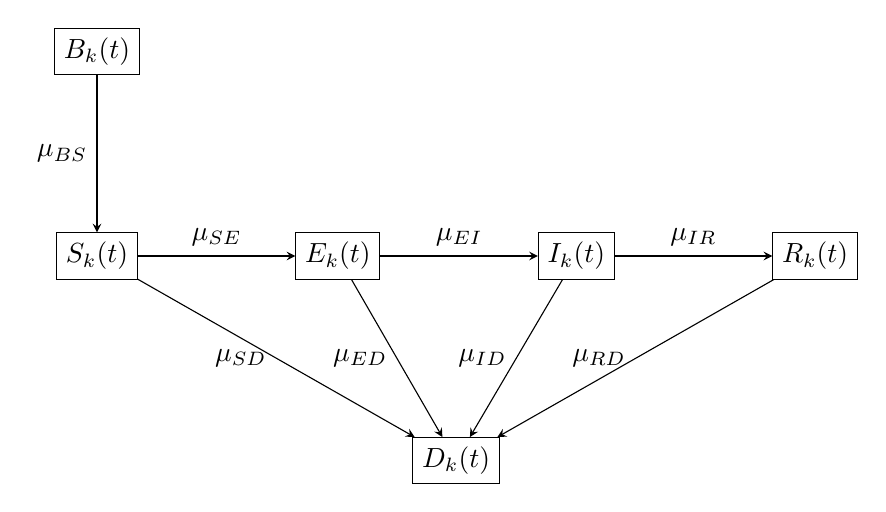
\begin{tikzpicture}[node distance=2cm, auto, >=stealth]
        % Nodes
        \node [draw, rectangle] (B) {$B_{k}(t)$};
        \node [draw, rectangle, below=of B] (S) {$S_{k}(t)$};
        \node [draw, rectangle, right=of S] (E) {$E_{k}(t)$};
        \node [draw, rectangle, right=of E] (I) {$I_{k}(t)$};
        \node [draw, rectangle, right=of I] (R) {$R_{k}(t)$};

        % “Dead” node positioned below E with an x-shift
        \node [draw, rectangle, below=2cm of E, xshift=1.5cm] (D) {$D_{k}(t)$};

        % Arrows with labels
        \draw[->] (B) -- node[midway, left] {{$\mu_{BS}$}} (S);
        \draw[->] (S) -- node[midway] {$\mu_{SE}$} (E);
        \draw[->] (E) -- node[midway] {$\mu_{EI}$} (I);
        \draw[->] (I) -- node[midway] {$\mu_{IR}$} (R);

        \draw[->] (S) -- node[left] {$\mu_{SD}$} (D);
        \draw[->] (E) -- node[left] {$\mu_{ED}$} (D);
        \draw[->] (I) -- node[left] {$\mu_{ID}$} (D);
        \draw[->] (R) -- node[left] {$\mu_{RD}$} (D);
    \end{tikzpicture}
    \caption{Flow chart of the WWR model.}
\end{figure}

Measles data frequently arise from surveillance across $J=40$ geographically distinct yet interconnected cities. In each city $k$, we track four compartments at time $t$: 
\[
S_{k}(t)\; (\text{susceptible}),\quad 
E_{k}(t)\; (\text{exposed}),\quad 
I_{k}(t)\; (\text{infectious}),\quad
R_{k}(t)\; (\text{recovered}).
\]
Their initial values $S_{k,0},E_{k,0},I_{k,0},R_{k,0}$ can be drawn from a multinomial distribution:
\[
\begin{bmatrix}
S_{k,0} & E_{k,0} & I_{k,0} & R_{k,0}
\end{bmatrix}
\sim
\mathrm{Mult}\bigl(n_{k,0}, \boldsymbol{\pi}_{k,0}\bigr).
\]

Over time, the model evolves via:
\[
\begin{alignedat}{2}
    S_{k,t+1} &= S_{k,t} - B_{k,t} - F^{(S)}_{k,t} + A_{k,t},\\ 
    E_{k,t+1} &= E_{k,t} + B_{k,t} - C_{k,t} - F^{(E)}_{k,t},\\
    I_{k,t+1} &= I_{k,t} + C_{k,t} - D_{k,t} - F^{(I)}_{k,t},\\
    R_{k,t+1} &= R_{k,t} + D_{k,t} - F^{(R)}_{k,t}.
\end{alignedat}
\]
Here, $B_{k,t}$ is the number of new infections in city $k$ at time $t$, modeled as
\[
B_{k,t}
\sim 
\mathrm{Bin}\Bigl(S_{k,t} - F^{(S)}_{k,t},\;1 - \exp[-h\,b_{k,t}]\Bigr),
\]
where $h$ is a discrete time step and $b_{k,t}$ is the within- plus between-city transmission rate. Specifically,
\[
b_{k,t}
=
\beta_{k,t}\,\xi_{k,t}
\times
\Bigl[
  \Bigl(\tfrac{I_{k,t}}{n_{k,t}}\Bigr)
  \;+\; 
  \sum_{l \neq k} \frac{v_{k,l}}{n_{k,t}}\Bigl(
    \bigl(\tfrac{I_{l,t}}{n_{l,t}}\bigr)
    \;-\;
    \bigl(\tfrac{I_{k,t}}{n_{k,t}}\bigr)
  \Bigr)
\Bigr].
\]
Here, $\beta_{k,t}$ captures the seasonal transmission for city $k$, $\xi_{k,t}\sim \mathrm{Gamma}(\sigma_{\xi},\sigma_{\xi})$ is a mean-one overdispersion factor, and $v_{k,l}$ reflects the coupling between cities $k$ and $l$. Often, $\beta_{k,t}$ alternates between school-term and holiday values:
\[
\beta_{k,t}
=
\begin{cases}
(1 + 2(1-p)\,a)\,\overline{\beta}_{k}, & \text{if in school term},\\
(1 - 2\,p\,a)\,\overline{\beta}_{k}, & \text{if in holiday},
\end{cases}
\]
where $\overline{\beta}_{k}$ is the average transmission rate, $p$ is the fraction of the year spent in school, and $a$ is the amplitude of the holiday effect.

Demographic processes such as births and deaths can be incorporated by defining
\[
\boldsymbol{\delta}_{k,t} 
= 
[\delta_{k,t}^{(S)},\,\delta_{k,t}^{(E)},\,\delta_{k,t}^{(I)},\,\delta_{k,t}^{(R)}]^\top 
\quad\text{and}\quad
\boldsymbol{\alpha}_{k,t}
= 
[\alpha_{k,t}^{(1)},\,0,\,0,\,0]^\top,
\]
so that
\[
F_{k,t}^{(\cdot)} 
\sim 
\mathrm{Bin}\bigl((\cdot)_{k,t},\,1 - \delta_{k,t}^{(\cdot)}\bigr),\quad
A_{k,t} 
\sim
\mathrm{Pois}(\alpha_{k,t}^{(1)}).
\]
Each city’s transitions can be encoded in a $4\times4$ matrix for particle filtering:
\[
\mathbf{K}_{r,\boldsymbol{\eta},\xi,k}
=
\begin{bmatrix}
e^{-h\,g_k(\beta_{k,r},\boldsymbol{\eta},\xi)} 
  & 1 - e^{-h\,g_k(\beta_{k,r},\boldsymbol{\eta},\xi)} 
  & 0 & 0\\
0 & e^{-h\,\rho} & 1 - e^{-h\,\rho} & 0\\
0 & 0 & e^{-h\,\gamma} & 1 - e^{-h\,\gamma}\\
0 & 0 & 0 & 1
\end{bmatrix},
\]
and realized transitions are arranged into a matrix $\mathbf{Z}_{k,t}$. By stacking these blocks across all $J$ cities, one obtains a $(4J)\times(4J)$ transition matrix, which is helpful for block particle filtering or other inference methods.

\subsection*{Multiple-Units Measles Model: Discrete Time Step}

For a discrete-time version, we similarly define the inter-city interaction:
\[
b_{k,\textcolor{red}{r}}
=
\beta_{k,\textcolor{red}{r}}\,\xi_{k,\textcolor{red}{r}}
\times
\Bigl[
  \Bigl(\tfrac{I_{k,\textcolor{red}{\tau_{r}}}}{n_{k,\textcolor{red}{\tau_{r}}}}\Bigr)
  \;+\; 
  \sum_{l \neq k} \frac{v_{k,l}}{n_{k,\textcolor{red}{\tau_{r}}}}\Bigl(
    \bigl(\tfrac{I_{l,\textcolor{red}{\tau_{r}}}}{n_{l,\textcolor{red}{\tau_{r}}}}\bigr)
    \;-\;
    \bigl(\tfrac{I_{k,\textcolor{red}{\tau_{r}}}}{n_{k,\textcolor{red}{\tau_{r}}}}\bigr)
  \Bigr)
\Bigr].
\]
The other transitions (e.g., births and deaths) can be similarly embedded in each discrete interval. This setup handles aggregated incidence over blocks $\tau_{r-1}+1$ to $\tau_r$ just as in the Euler step framework, but now with a single gamma draw per longer interval. Such discrete-time constructions also allow additional extension for background importations or other city-specific processes.

\section{\texorpdfstring{$\fmeas$}{fmeas}: Measurement model for filter}

We now describe the measurement models associated with the filter. Under $\fmeas=\fmeasBinomial$, observations are treated as binomial draws with potentially overdispersed multiplicative noise on the underlying reporting probability. In contrast, $\fmeas=\fmeasGaussian$ uses a discretized Gaussian likelihood for measurement. Both forms permit tractable likelihood computation without requiring expensive Monte Carlo integration. In practice, the basic PAL method necessitates a binomial-style measurement process, but its SMC-PAL extension also accommodates stochastic variation in the measurement probability.

\subsection*{Gaussian Model}

Here, we account for both under-reporting and measurement error. Specifically, we set
\[
\mathbb{E}[Y_{k,t}^{(3,4)} \mid D_{k,t}] = \rho_{meas}\,D_{k,t},
\]
where $0 < \rho_{meas} < 1$ is the reporting efficiency and $D_{k,t}$ is the true number of infective-to-recovered transitions. We assume
\[
\mathrm{Var}[Y_{k,t}^{(3,4)} \mid D_{k,t}] 
= \rho_{meas}\,\bigl(1 - \rho_{meas}\bigr)\,D_{k,t} 
\;+\; 
\bigl(\psi\,\rho_{meas}\,D_{k,t}\bigr)^{2},
\]
where $\psi$ governs overdispersion. When $\psi=0$, this reduces to the usual binomial variance-mean relationship. We then posit a discretized normal likelihood:
\[
\begin{aligned}
f\bigl(y_{k,t}^{(3,4)} \mid \rho_{meas},\psi,D_{k,t}\bigr)
&=
\Phi\Bigl(
  y_{k,t}^{(3,4)} + \tfrac{1}{2},\rho_{meas}\,D_{k,t},\\
&\quad
  \rho_{meas}(1-\rho_{meas})\,D_{k,t}
    + (\psi\,\rho_{meas}\,D_{k,t})^{2}
\Bigr)\\
&\quad-\;
\Phi\Bigl(
  y_{k,t}^{(3,4)} - \tfrac{1}{2},
  \rho_{meas}\,D_{k,t},\\
&\quad
  \rho_{meas}(1-\rho_{meas})\,D_{k,t}
    + (\psi\,\rho_{meas}\,D_{k,t})^{2}
\Bigr).
\end{aligned}
\]

where $\Phi(\cdot,\mu,\sigma^2)$ is the c.d.f.\ of a normal distribution with mean $\mu$ and variance $\sigma^2$.

\subsection*{Binomial Model}

In the binomial measurement model, we observe the aggregated number of infections removed (i.e., transitions from infective to recovered) over each two-week interval. Writing
\[
\overline{Y}_{k,r} \;=\; \sum_{t=\tau_{r-1}+1}^{\tau_r} Y_{k,t},
\]
we assume 
\[
Y_{k,t}^{(3,4)} \;\sim\; \mathrm{Bin}\bigl(D_{k,t},\,Q_{k,r}^{(3,4)}\bigr),
\]
with $D_{k,t}$ the true infective-to-recovered counts at time $t$ and $Q_{k,r}^{(3,4)}$ the reporting probability during interval $r$. This rate $Q_{k,r}^{(3,4)}$ follows a normal distribution truncated to $[0,1]$. In practice, we set the means $\mu_{q,k}$ to known prior estimates for each city, leaving $\sigma_q^2$ to be inferred from the data.  

\section{F: Filter algorithm}

Below, we provide pseudo-code for three filtering methods central to our analyses. 

\begin{algorithm}[H]
\caption{bpfilter(\texttt{P}, \texttt{Np}=J, \texttt{block\_list}=$\mathcal{B}$). This block particle filter uses the notation of Table~1. The object \texttt{P} is a ‘spatPomp’ object providing \texttt{rprocess}, \texttt{dunit\_measure}, \texttt{rinit}, \texttt{obs}, \texttt{coef}.}
\begin{algorithmic}[1]
\REQUIRE simulator for $f_{X_n|X_{n-1}}(x_n | x_{n-1}; \theta)$ and $f_{X_0}(x_0; \theta)$; number of particles, $J$; evaluator for $f_{Y_{u,n}|X_{u,n}}(y_{u,n} | x_{u,n}; \theta)$; data, $\mathbf{y}_{1:N}^*$; parameter, $\theta$; blocks, $\mathcal{B}_{1:K}$

\STATE initialization, $X_0^{F,j} \sim f_{X_0}(\cdot; \theta)$ for $j$ in $1:J$
\FOR{$n$ in $1:N$}
    \STATE prediction, $X_n^{P,j} \sim f_{X_n|X_{n-1}}(\cdot | X_{n-1}^{F,j}; \theta)$ for $j$ in $1:J$
    \FOR{$k$ in $1:K$}
        \STATE block weights, $w_k^{j,n} = \prod_{u \in \mathcal{B}_k} f_{Y_{u,n}|X_{u,n}}(y_{u,n}^* | X_{u,n}^{P,j}; \theta)$ for $j$ in $1:J$
        \STATE resampling indices, $r_k^{j,n}$ with $\mathbb{P}\bigl[r_k^{j,n} = i\bigr] = \dfrac{w_k^{i,n}}{\sum_{q=1}^J w_k^{q,n}}$ for $j$ in $1:J$
        \STATE resample, $X_{\mathcal{B}_k,n}^{F,j} = X_{\mathcal{B}_k,n}^{P,\,r_k^{j,n}}$ for $j$ in $1:J$
    \ENDFOR
\ENDFOR
\ENSURE output: log-likelihood, $\lambda^{BPF}(\theta) = \sum_{n=1}^N \sum_{k=1}^K \log\left(\tfrac{1}{J} \sum_{j=1}^J w_k^{j,n}\right)$, filter particles $X_{1:N}^{F,1:J}$
\end{algorithmic}
\end{algorithm}


\begin{algorithm}[H]
\caption{The IBPF algorithm (iterated block particle filter).}
\begin{algorithmic}[1]
\REQUIRE Initial value function $f_{X_0}(\theta)$; 
simulator for $f_{X_n|X_{n-1}}(x_n | x_{n-1}; \theta)$, $n \in 1:N$; 
evaluator for $f_{Y_n|X_n}(y_n | x_n; \theta)$, $n \in 1:N$; 
data, $\mathbf{y}_{1:N}$; 
number of iterations, $M$; 
number of particles, $J$; 
partition, $K$; 
initial parameter swarm, $\{\Theta_0^0, j \in 1:J\}$; 
perturbation density, $f_{\theta_n|\theta_{n-1}}(\theta_n | \vartheta; \sigma)$, $n \in 1:N$; 
perturbation sequence, $\sigma_{1:M}$.

\ENSURE Final parameter swarm, $\{\Theta_j^M, j \in 1:J\}$ and log-likelihood $\hat{\ell}_b$.

\FOR{m in 1:M}
    \STATE Set $\Theta_{0,j}^{F,m} = \Theta_{j}^{m-1}$ for $j \in 1:J$.
    \STATE Set $X_{0,j}^{F,m} = f_{X_0}(\Theta_{0,j}^{F,m})$ for $j \in 1:J$.
    \FOR{n in 1:N}
        \STATE Draw $\Theta_{n,j}^{P,m} \sim f_{\theta_n|\theta_{n-1}}(\theta_n | \Theta_{n-1,j}^{F,m}; \sigma_m)$ for $j \in 1:J$.
        \STATE Draw $X_{n,j}^{P,m} \sim f_{X_n|X_{n-1}}(x_n | X_{n-1,j}^{F,m}; \Theta_{n,j}^{P,m})$ for $j \in 1:J$.
        \FOR{$K \in \mathcal{K}$}
            \STATE Compute $w_{n,j}^{K,m} = \prod_{s \in K} f_{Y_s|X_s}(y_s^u | X_s^u, \Theta_{n,j}^{P,m})$ for $j \in 1:J$.
            \STATE Draw $s_{n,j}^{K,m}$ with $\mathrm{Prob}(s_{n,j}^{K,m} = i) = \dfrac{w_{n,i}^{K,m}}{\sum_{j=1}^J w_{n,j}^{K,m}}$ for $j \in 1:J$.
        \ENDFOR
        \STATE Set $X_{n,j}^{F,m} = (X_{n,j}^{K,F,m})_{K \in \mathcal{K}}$ where $X_{n,j}^{K,F,m} = X_{n,s_{n,j}^{K,m}}^{K,P,m}$ for $j \in 1:J$.
        \STATE Set $\Theta_{n,j}^{F,m} = (\Theta_{n,j}^{K,F,m})_{K \in \mathcal{K}}$ where $\Theta_{n,j}^{K,F,m} = \Theta_{n,s_{n,j}^{K,m}}^{K,P,m}$ for $j \in 1:J$.
    \ENDFOR
    \STATE Set $\Theta_{j}^{m} = (\Theta_{n,j}^{F,m})_{n \in 1:N}$ for $j \in 1:J$.
\ENDFOR
\STATE Set $\hat{\ell}_b = \sum_{n=1}^N \sum_{K \in \mathcal{K}} \log \left( \frac{1}{J} \sum_{j=1}^J w_{n,j}^{K,m} \right)$.
\end{algorithmic}
\end{algorithm}

\begin{algorithm}[H]
\caption{PAL within a lookahead block particle filter}\label{alg:measles_block_lookahead}
\begin{algorithmic}[1]

\STATE {\bf Initialize:} Set $\bar{\bs \lambda}_{0,k}^{(i)} \leftarrow  n_{k,0} \bs \pi_{k,0}$, 
  $\log \zeta_{0,k}^{(i)} \leftarrow 0$, 
  and $\log W_{0,k}^{(i)} \leftarrow 0$ 
  for $i = 1$ to $n_{part}$ and $k = 1, \dots, K.$

\FOR{$r \geq 1$}
  \FOR{$k = 1, \dots, J$}
    \FOR{$i = 1, \dots, n_{part}$}
      \STATE $\xi_{k,r}^{(i)} \sim \mathrm{Gamma}(\sigma_{\xi}, \sigma_{\xi})$
      \FOR{$t = \tau_{r-1} + 1, \dots, \tau_r - 1$}
        \STATE $\bs \Lambda_{t,k}^{(i)} \leftarrow  
           \Bigl((\bar{\bs \lambda}^{(i)}_{t-1,k} \circ \bs \delta_{t,k}) 
           \otimes \+1_m\Bigr)
           \;\circ\;
           \+K_{r,\bs \eta\bigl(\bar{ \bs \lambda}_{\tau_{r-1},1:J}^{(i)}\bigr),\,
                \xi_{k,r}^{(i)},\,k}$
        \STATE $\bar{\bs \lambda}^{(i)}_{t,k} \leftarrow  
            (\+1_m^\top \bs \Lambda_{t,k}^{(i)})^\top + \bs \alpha_{t,k}$
      \ENDFOR

      \STATE $\bs \Lambda^{(i)}_{\tau_r,k} \leftarrow  
          \Bigl((\bs \lambda^{(i)}_{\tau_r -1,k} \circ \bs \delta_{\tau_r,k}) 
          \otimes \+1_m\Bigr)
          \;\circ\;
          \+K_{r,\bs \eta\bigl(\bar{ \bs \lambda}_{\tau_{r-1},1:J}^{(i)}\bigr),\,
                \xi_{r,k}^{(i)},\,k}$
      \STATE $\+Q_{k,r}^{(i)} \sim \pi\Bigl(\cdot \,\middle|\,
           \{\bs \Lambda^{(i)}_{t,k}\}_{t = \tau_{r-1}+1}^{\tau_{r}},\,
           \bar{\+ Y}_{r,k},\,
           \bs \varphi
        \Bigr)$
      \STATE $\+M_{r,k}^{(i)} \leftarrow  
          \sum_{t = \tau_{r-1}+1}^{\tau_{r}} 
            \bs \Lambda^{(i)}_{t,k} \,\circ\, \+Q_{k,r}^{(i)}$
      \STATE $\mathcal{L}(\bar{\+ Y}_{r,k} \mid \bar{\+ Y}_{1:r-1,k} ) 
         \leftarrow  
           -\,\+1_m^\top \+M_{r,k}^{(i)} \+1_m 
           \;+\; \+1_m^\top\bigl(\bar{\+ Y}_{r,k}\,\circ\,\log \+M_{r,k}^{(i)}\bigr)\+1_m 
           \;-\; \+1_m^\top\bigl(\log \bar{\+Y}_{r,k}!\bigr)\+1_m$
      \STATE $\log w^{(i)}_{r,k} \leftarrow 
          \mathcal{L}(\bar{\+ Y}_{r,k} \mid \bar{\+ Y}_{1:r-1,k} ) 
          + \log\Bigl(f(\+Q_{k,r}^{(i)} \mid \+Q_{k,1:r-1}^{(i)})\Bigr) 
          - \log\Bigl(\pi\bigl(\+Q_{k,r}^{(i)} \,\mid\, 
            \{\bs \Lambda^{(i)}_{t,k}\}_{t = \tau_{r-1}+1}^{\tau_{r}}, 
            \bar{\+ Y}_{r,k}, 
            \bs \varphi \bigr)\Bigr)$
      \STATE $\bar W_{r-1,k}^{(i)} \leftarrow 
          \dfrac{W_{r-1,k}^{(i)}}{\sum_j W_{r-1,k}^{(j)}} 
          \quad (i = 1 \dots n_{part})$
      \STATE $\log W_{r,k}^{(i)} \leftarrow 
          \log \bar W_{r-1,k}^{(i)} + \log w_{r,k}^{(i)}$
      \STATE $\bar{\bs \Lambda}^{(i)}_{\tau_r,k} \leftarrow
          (\+1_m \otimes \+1_m - \+Q_{k,r}^{(i)}) \,\circ\, \bs \Lambda_{\tau_r,k}
          \;+\;
          \bar{\+Y}_{r,k} \,\circ\, \bs \Lambda_{\tau_r,k}^{(i)} 
          \,\circ\, \+Q_{k,r}^{(i)} \,\oslash\, \+M_{r,k}^{(i)}$
      \STATE $\bar{\bs \lambda}^{(i)}_{\tau_r,k} \leftarrow 
          \bigl(\+1_m^\top \bar{\+ \Lambda}^{(i)}_{\tau_r,k}\bigr)^\top 
          + \bs \alpha_{\tau_r,k}$
    \ENDFOR
  \ENDFOR

  \FOR{$k = 1, \dots, J$}
    \FOR{$i = 1, \dots, n_{part}$}
      \STATE $\tilde{\xi}_{k,r+1}^{(i)} \sim \mathrm{Gamma}(\sigma_{\xi}, \sigma_{\xi})$
      \FOR{$t = \tau_r + 1, \dots, \tau_{r+1} - 1$}
        \STATE $\bs \Lambda_{t,k}^{(i)} \leftarrow  
            \Bigl((\bar{\bs \lambda}^{(i)}_{t-1,k} \circ \bs \delta_{t,k}) 
            \otimes \+1_m\Bigr)
            \;\circ\;
            \+K_{r+1,\bs \eta\bigl(\bar{\bs \lambda}_{\tau_r,1:J}^{(i)}\bigr),\,
                  \tilde{\xi}_{r+1,k}^{(i)},\,k}$
        \STATE $\bar{\bs \lambda}^{(i)}_{t,k} \leftarrow  
            (\+1_m^\top \bs \Lambda_{t,k}^{(i)})^\top + \bs \alpha_{t,k}$
      \ENDFOR
      \STATE $\bs \Lambda^{(i)}_{\tau_{r+1},k} \leftarrow  
          \Bigl((\bs \lambda^{(i)}_{\tau_{r+1}-1,k} \circ \bs \delta_{\tau_{r+1},k}) 
          \otimes \+1_m\Bigr)
          \;\circ\;
          \+K_{r+1,\bs \eta\bigl(\bar{\bs \lambda}_{\tau_r,1:J}^{(i)}\bigr),\,
                \tilde{\xi}_{r+1,k}^{(i)},\,k}$
      \STATE $\tilde{\+Q}_{k,r+1}^{(i)} \sim \pi\Bigl(\cdot \,\middle|\,
          \{\bs \Lambda^{(i)}_{t,k}\}_{t = \tau_r+1}^{\tau_{r+1}},\,
          \bar{\+ Y}_{r+1,k},\,
          \bs \varphi 
        \Bigr)$
      \STATE $\+M_{r+1,k}^{(i)} \leftarrow  
          \sum_{t = \tau_r + 1}^{\tau_{r+1}} 
            \bs \Lambda^{(i)}_{t,k} \,\circ\, \tilde{\+Q}_{r+1,k}^{(i)}$
      \STATE $\mathcal{L}(\bar{\+ Y}_{r+1,k} \mid \bar{\+ Y}_{1:r,k} ) 
         \leftarrow  
           -\,\+1_m^\top \+M_{r+1,k}^{(i)} \+1_m 
           \;+\; \+1_m^\top \bigl(\bar{\+ Y}_{r+1,k}\,\circ\,\log \+M_{r+1,k}^{(i)}\bigr)\+1_m 
           \;-\; \+1_m^\top \bigl(\log \bar{\+Y}_{r+1,k}!\bigr)\+1_m$
      \STATE $\log w^{(i)}_{r+1,k} \leftarrow 
          \mathcal{L}(\bar{\+ Y}_{r+1,k} \mid \bar{\+ Y}_{1:r,k} )
          + \log\Bigl(f(\+Q_{k,r+1}^{(i)} \mid \+Q_{k,1:r}^{(i)})\Bigr)
          - \log\Bigl(\pi\bigl(\+Q_{k,r+1}^{(i)} 
            \,\mid\, 
            \{\bs \Lambda^{(i)}_{t,k}\}_{t = \tau_r+1}^{\tau_{r+1}}, 
            \bar{\+ Y}_{r+1,k}, 
            \bs \varphi 
          \bigr)\Bigr)$
      \STATE $\log \zeta_{r,k}^{(i)} \leftarrow 
          \log W_{r,k}^{(i)} + \log w_{r+1,k}^{(i)}$
    \ENDFOR

    \STATE $\hat{\mathcal{L}}(\bar{\+ Y}_{r,k} \mid \bar{\+ Y}_{1:r-1,k} ) 
       \leftarrow 
         \log\Bigl(\sum_j W_{r,k}^{(j)}\Bigr)$
    \STATE $\bar \zeta_{r,k}^{(i)} \leftarrow 
        \dfrac{\zeta_{r,k}^{(i)}}{\sum_j \zeta_{r,k}^{(j)}} 
        \quad (i = 1 \dots n_{part})$
    \STATE {\bf Resample} 
      $\bigl\{\bar{\bs \lambda}^{(i)}_{\tau_r, k},\, W_{r,k}^{(i)},\, \zeta_{r,k}^{(i)}\bigr\}_{i=1}^{n_{part}}$
      with weights $\{\bar{\zeta}_{r,k}^{(i)}\}_{i=1}^{n_{part}}$
    \STATE $\log W_{r,k}^{(i)} \leftarrow 
        \log W_{r,k}^{(i)} \;-\; \log \zeta_{r,k}^{(i)}$
  \ENDFOR
\ENDFOR

\end{algorithmic}
\end{algorithm}
\end{document}

